%! TEX program = xelatex
% WARNING: this is a generated file.
%
% Please do not edit this file directly. 
% - If you want to update the medatata of the paper (title, authors, abstract), please
%   edit the `paper-meta.yaml` file in the root of the repository.
% - If you want to update the content of the paper, please edit the latex files
%   in the `src` directory.
% - If you want to update the template itself (e.g., change the layout), please
%   edit the `templates/lipics/lipics.tex` file instead.
\documentclass[
    a4paper,
    UKenglish,
    cleveref,
    autoref,
    thm-restate]{lipics-v2021}

\usepackage{todonotes}
\usepackage{lineno}
\linenumbers




% math packages
\usepackage{stmaryrd,thmtools,upgreek}
\usepackage{amsmath,amssymb,amsfonts}

% graphics packages
\usepackage{graphicx}
\usepackage[obeyclassoptions,mode=tex]{standalone}
\usepackage{tikz}
\usetikzlibrary{backgrounds}
\usetikzlibrary{calc}
\usetikzlibrary{shapes.geometric}
\usetikzlibrary{positioning}
\usetikzlibrary{automata}
\usetikzlibrary{tikzmark}
\usetikzlibrary{patterns}
\usetikzlibrary{arrows}
\tikzset{every state/.style={minimum size=1pt}}
\usepackage{tikz-cd}


% links inside the document
\usepackage[composition,hyperref,xcolor,cleveref]{knowledge}
\knowledgeconfigure{notion}

% Tables 
\usepackage{booktabs}
\usepackage{varwidth}

% Packages for macro definitions
\usepackage{xparse}
\usepackage{xpatch}
\usepackage{tokcycle}
\usepackage{ifthen}

% Proofs
\usepackage{bussproofs}

% Colors 
\usepackage{ensps-colorscheme}


% we include whatever the user wants to include in the header

% we include libraries (tex files) usually written in the `lib` directory
\input{lib/aliaume.tex}

\NewDocumentCommand{\Cls}{}{\mathcal{C}}

\NewDocumentCommand{\Label}{ m m }{\mathsf{Label}_{#1}(#2)}
\NewDocumentCommand{\treeRoot}{}{\mathsf{root}}
\NewDocumentCommand{\lca}{}{\mathop{\mathsf{lca}}}

\NewDocumentCommand{\treeleq}{ O{} }{\sqsubseteq_{#1}}
\NewDocumentCommand{\treelt}{ O{} }{\sqsubset_{#1}}
\NewDocumentCommand{\Trees}{ m }{\mathsf{Trees}_{#1}}
\NewDocumentCommand{\Leaves}{ m }{\mathsf{Leaves}(#1)}
\NewDocumentCommand{\Graphs}{ O{} }{\mathsf{Graphs}_{#1}}

\NewDocumentCommand{\tlbl}{ m m m }{ [{#2}{\colon}\!{#3}]_{#1}}


\NewDocumentCommand{\cmpleq}{}{\preceq}
\NewDocumentCommand{\cmplt}{}{\prec}

\NewDocumentCommand{\isubleq}{}{\subseteq_i}
\NewDocumentCommand{\isublt}{}{\subset_i}

% Projections on a branch
\NewDocumentCommand{\Br}{}{\mathop{\mathsf{B}_r}}
\NewDocumentCommand{\Bl}{}{\mathop{\mathsf{B}_l}}
\NewDocumentCommand{\Bt}{}{\mathop{\mathsf{B}_t}}

% Monoid labels based on a branch
\NewDocumentCommand{\BrL}{}{\mathop{\mu_{\mathsf{B}}^r}}
\NewDocumentCommand{\BlL}{}{\mathop{\mu_{\mathsf{B}}^l}}
\NewDocumentCommand{\BtL}{}{\mathop{\mu_{\mathsf{B}}^t}}

\NewDocumentCommand{\spt}{}{\mathfrak{s}}

\NewDocumentCommand{\aTree}{O{T}}{\mathcal{#1}}

\newcommand{\existsu}{\exists!}

\input{lib/knowledges.kl}

% We include the title and author information based on the 
% `paper-meta.yaml` file.
 
\title{Well-quasi-ordered classes of bounded clique-width}

\author{Aliaume Lopez}
       {INP Bordeaux, LaBRI, CNRS}
       {aliaume.lopez@bordeaux-inp.fr}
       {https://orcid.org/0000-0002-4205-327X}
       {}
\author{Maël Dumas}
       {University of Warsaw}
       {m.dumas2@uw.edu.pl}
       {}
       {}

\authorrunning{A. Lopez and M. Dumas}

\Copyright{Aliaume Lopez and Maël Dumas} 

\ccsdesc[100]{Formal languages and automata theory}
\ccsdesc[100]{Graph theory}

\keywords{well-quasi-ordering, clique-width, automata theory, monoids, factorization forests, gap embedding} %TODO mandatory; please add comma-separated list of keywords

\category{} %optional, e.g. invited paper




\newcommand{\repositoryUrl}{\url{}}

%Editor-only macros:: begin (do not touch as author)%%%%%%%%%%%%%%%%%%%%%%%%%%%%%%%%%%
\EventEditors{John Q. Open and Joan R. Access}
\EventNoEds{2}
\EventLongTitle{42nd Conference on Very Important Topics (CVIT 2016)}
\EventShortTitle{CVIT 2016}
\EventAcronym{CVIT}
\EventYear{2016}
\EventDate{December 24--27, 2016}
\EventLocation{Little Whinging, United Kingdom}
\EventLogo{}
\SeriesVolume{42}
\ArticleNo{23}
%%%%%%%%%%%%%%%%%%%%%%%%%%%%%%%%%%%%%%%%%%%%%%%%%%%%%%

% Now, we create the document itself.
\begin{document}
% Generate the title page
\maketitle
% Print the abstract
\begin{abstract}
    We study classes of graphs with bounded clique-width that are well-quasi-ordered by the induced subgraph relation, in the presence of labels on the vertices. We prove that, given a finite presentation of a class of graphs, one can decide whether the class is labelled-well-quasi-ordered. This solves an open problem raised by Daligault, Rao and Thomassé in 2010. From our proof techniques, we also derive (restricted versions of) conjectures of Pouzet regarding well-quasi-ordering of graphs under the induces subgraph relation. Finally, we provide a structural characterization of those classes as those that are of bounded clique-width and do not existentially transduce the class of all finite paths.
\end{abstract}

% Include the content of the paper

\section{Introduction}
\label{sec:introduction}

\AP A quasi-ordered set $(X, \leq)$ is \intro{well-quasi-ordered} (WQO) if
every non-empty subset of $X$ has a finite non-empty subset $Y \subfin X$ of
minimal elements, i.e. such that for every $x \in X$, there exists $y \in Y$
such that $y \leq x$. When the set $X$ is totally ordered, this is equivalent
to the usual notion of well-ordering, but in the presence of incomparable
elements, it is a stronger condition. The theory of well-quasi-orderings (WQOs)
is a powerful combinatorial setting that has found applications in various
areas of mathematics and computer science. In graph theory, the celebrated
result of Robertson and Seymour~\cite{ROBSEY04} states that the class of all
finite graphs is well-quasi-ordered under the minor relation, a profound result
with deep algorithmic consequences. WQOs are also at the heart of
\emph{well-structured transition systems}, infinite state transitions systems
over which verification algorithms can be designed~\cite{ABDU96,ABDU98}. One of
the appeal of WQOs is that they are closed under various operations, such as
the sum and the product of WQOs. As an example, the closure of WQOs under the
finite words, also known as Higman's lemma \cite{HIG52}, has been used in the
verification of so-called \emph{lossy channel systems}~\cite{ABDU93}. 


% Well-quasi-ordered classes of graphs
\AP Undirected finite graphs are naturally equipped with the \reintro{induced
subgraph relation}, where $G$ is an induced subgraph of $H$ if $G$ can be
obtained from $H$ by deleting vertices (and the edges adjacent to them). Unlike
the graph minor relation, the induced subgraph relation is not a
well-quasi-ordering on the class of all finite graphs, as witnessed by the
infinite family of cycles of increasing size, which form an infinite antichain.
However, some classes of finite graphs are well-quasi-ordered under the induced
subgraph relation: for instance, the class of all finite paths, or the class of
all finite cliques. Distinguishing which classes of finite graphs are
well-quasi-ordered under the induced subgraph relation is a long-standing open
problem in graph theory, dating back to Pouzet's seminal work \cite{POUZ72}.

\AP In general, there is little hope to characterise all such classes, since
any countable order with finite infixes can be embedded into the induced
subgraph relation on finite graphs (this is a consequence of \cite[Lemma
5.1]{Kuske06}). However, there are high hopes that a better notion of
well-quasi-ordering on classes of finite graphs is more amenable to structural
characterisations. This is why one usually considers \emph{labelled}
well-quasi-orderings on classes of finite graphs. Given a class $\Cls$ of
finite graphs, and a well-quasi-ordering $(X, \leq)$, one can consider the
class $\Label{X}{\Cls}$ of graphs in $\Cls$ whose vertices are labelled by
elements of $X$. The induced subgraph relation is then extended to labelled
graphs by requiring that the labels are preserved by the embedding, i.e. that
the label of a vertex in the smaller graph is less than or equal to the label
of its image in the larger graph. 

\begin{example}
  \label{ex:labelled-graphs}
  The class of all finite paths is not $2$-well-quasi-ordered,
  since the infinite sequence of paths with colored endpoints 
  forms an infinite antichain.
  The class of cliques is labelled-well-quasi-ordered,
  since any labelled clique can be identified with a multiset of labels,
  and the set of finite multisets over a WQO is itself WQO.
\end{example}


\AP
Bounded clique-width is a well-studied graph complexity measure
that generalises other well-known graph complexity measures such as
todo. There are several equivalent definitions of 
having \emph{bounded clique-width}, and we will use two 
of them in this paper. On the one hand, a class of graphs $\Cls$ has
\emph{bounded clique-width} if it is MSO-transducable from a class of finite
trees. On the other hand, a class of graphs $\Cls$ has 
\emph{bounded clique-width} if there exists a finite set of 
labels $\Sigma$ such that 
every graph in $\Cls$ can be constructed using the following operations:
\begin{itemize}
  \item creating a new vertex with label $a \in \Sigma$,
  \item taking the disjoint union of two labelled graphs,
  \item adding edges between all vertices of label $a$ and all vertices of label $b$,
  \item renaming all labels $a$ into $b$.
\end{itemize}

\begin{example}
  The class of all finite cliques, finite paths, finite cycles, 
  and finite trees all have bounded clique-width.
\end{example}

\begin{example}
  The class of all finite grids does not have bounded clique-width.
\end{example}



\paragraph*{Contributions}
\AP
We prove that one can decide whether a class of graphs of bounded clique-width
is labelled-well-quasi-ordered, when the class is given by
an $\MSO$ interpretation from finite trees to undirected graphs.
Our proof scheme 




\paragraph*{Related works}

There are three natural conjectures that have been formulated 
regarding the relationship between various notions of well-quasi-ordering on
classes of finite graphs.

\begin{conjecture}[Pouzet \cite{POUZ72}]
    \label{pouzet:conj}
    Let $\Cls$ be a class of finite graphs.
    Then, the following are equivalent:
    \begin{enumerate}
      \item $\Cls$ is pointed-well-quasi-ordered,
      \item $\Cls$ is 2-well-quasi-ordered,
      \item $\Cls$ is labelled-well-quasi-ordered,
      \item $\Cls$ is wqo-well-quasi-ordered.
      \item $\Cls$ one can add a total order on the vertices of 
        its graphs, and remain wqo-well-quasi-ordered.
    \end{enumerate}
\end{conjecture}

\begin{conjecture}[{\cite[Conjecture 4]{DRT10}}]
  \label{thomasse:conj}
  Let $\Cls$ be a hereditary class of finite graphs of bounded clique-width.
  Then, $\Cls$ is $2$-well-quasi-ordered if and only if
  there exists $\Cls \subseteq \Cls[D]$ 
  ``structurally simpler'' such that $\Cls[D]$ is $2$-well-quasi-ordered.
\end{conjecture}


\begin{conjecture}[\cite{ALM17}]
  \label{lozin:conj}
  Let $\Cls$ be a hereditary class of finite graphs that is not labelled-well-quasi-ordered.
  Then, there exists 
  an infinite bad sequence of graphs in $\Cls$
  that is \emph{regular}.
\end{conjecture}

\begin{conjecture}[Schmitz's Transduction Conjecture]
    \label{transduction:conj}
    Let $\Cls$ be a class of finite graphs.
    Then, $\Cls$ is labelled-well-quasi-ordered
    if and only if
    $\Cls$
    does not existentially transduce all finite paths.
\end{conjecture}


\begin{conjecture}[Szymon's Collapsing Conjecture]
    \label{nip-cw:conj}
    Let $\Cls$ be a class of graphs.
    If $\Cls$ is labelled-wqo,
    then $\Cls$ is of bounded clique-width.
\end{conjecture}

\paragraph*{Proof Techniques and Overview.} The overall proof technique can be
summarised in \cref{fig:proof-technique}. Given a class $\Cls$ of graphs
defined as the image of an $\MSO$ interpretation $I$ from finite trees to
graphs, we want to decide whether $\Cls$ is labelled-well-quasi-ordered. To
this end, we will use the following folklore result: if $(X, \leq)$ is a WQO,
and $f \colon X \to Y$ is a surjective order-preserving map, then $(Y, \leq)$
is also WQO. Because there exists a good candidate for $X$, namely, the set of
trees with Kruskal's tree embedding relation, we will try to see whether $I$ is
order-preserving. It turns out that for general interpretations, this is not
true (see \cref{example:msotree-not-monotone}). However, leveraging tools from
automata theory in the name of \emph{ramseyan factorisations} \cite{COLC07}, we
will be able to ``massage'' the input trees using a function $F$ into
\emph{nested trees}, with the property that for a good notion of ordering on
nested trees (nested Kruskal embedding essentially), the function $J$ that
factors $I$ through $F$ is order-preserving if and only if $\Cls$ is
labelled-well-quasi-ordered.

This proof technique will actually allow us to derive stronger results since it
shows that embeddings on graphs in $\Cls$ can be assumed to respect a certain
tree-like structure, and a fortiori, a linear order on the vertices of the
graphs. This will allow us to show that \cref{pouzet:conj} holds for classes of
graphs of bounded clique-width. Furthermore, listing the obstructions for $J$
to be order-preserving will allow us to show that counter-examples are regular
in nature, yielding a proof of \cref{lozin:conj} for classes of graphs of
bounded clique-width. Finally, the tree-like structure obtained is a form of
simple tree decomposition, answering positively to \cref{thomasse:conj} in
totality.


\paragraph*{Outline}



This explains the \emph{bottom-up} research direction in the field of WQOs,
which is to understand which \emph{constructors} preserve the WQO property:
finite sums, finite products, finite words, finite trees, finite graphs
\emph{with the minor relation} etc. It is motivated by the idea that one can
build complex orderings to model a concrete system by combining simpler ones,
and has empirically shown to be a fruitful approach (see \cite{HSS13} for an
example of nesting Higman's orderings). One other research direction is to
devise \emph{decision procedures} that take as input a set and decide whether
it is WQO or not, and whether classical decision algorithm on well-structured
transition systems can be applied to the concrete model one has. This dual
\emph{top-down} approach also had its recent share of successes
\cite{ALM17,FINGU19,LOPEZ24}.



\clearpage

\section{Preliminaries}
\label{sec:preliminaries}

\paragraph*{Graphs.} A \intro{graph} is a pair $G = (V, E)$ where $V$ is a set
of \intro{vertices} and $E \subseteq V \times V$ is a set of \intro{edges}. A
graph is \intro{undirected} if $(u, v) \in E$ implies $(v, u) \in E$ for all
$u, v \in V$. In this paper we will focus on finite undirected graphs. Given a
set $X$, an \intro{$X$-labelled graph} is a graph equipped with a function
$\ell \colon V \to X$ that assigns a label to each vertex. Given a class $\Cls$
of finite undirected graphs, write $\Label{X}{\Cls}$ for the class of freely
$X$-labelled graphs in $\Cls$, i.e., the class of all \kl{$X$-labelled graphs}
$G = (V, E, \ell)$ such that $G \in \Cls$.


\paragraph*{Well-quasi-orderings.} A quasi-ordered set $(X, \leq)$ is a set $X$
equipped with a reflexive and transitive relation $\leq$. A sequence
$\seqof{x_i}$ of elements in $X$ is \intro(sequence){good} if there exist $i <
j$ such that $x_i \leq x_j$. A quasi-ordered set is \intro{well-quasi-ordered}
(\reintro{wqo}) if every infinite sequence is \kl(sequence){good}.

\AP
Let $(X, \leq)$ be a quasi-order, and let $\Cls$ be a class of \kl{$X$-labelled
graphs}. Then, we define the \intro{$X$-induced quasi-order} on $\Cls$ as
follows: for $G, H \in \Cls$, we write $G \leq H$ if there exists a
\kl{monomorphism} $f \colon G \to H$ such that for all $v \in V$, we have
$\ell_G(v) \leq \ell_H(f(v))$. 

\AP A class $\Cls$ of finite undirected graphs is
\intro{labelled-well-quasi-ordered} (\reintro{labelled-wqo}) if for every
finite set $(X,=)$, the class $\Label{X}{\Cls}$ is \kl{well-quasi-ordered}
using the \kl{$X$-induced quasi-order}. A class of graph is
\intro{wqo-well-quasi-ordered} (\reintro{wqo-wqo}) if for every
\kl{well-quasi-order} $(X, \leq)$, the class $\Label{X}{\Cls}$ is
\kl{well-quasi-ordered} using the \kl{$X$-induced quasi-order}.

\paragraph*{Transductions.} An \intro{$\MSO$-interpretation} between two
classes $X$ and $Y$ of finite relational structures is given by formulii
$\phi_{\Delta}, \phi_{\delta}, \phi_{R}$ in \kl{monadic second-order logic}.
The interpretation defines a relation between structures of $X$ and $Y$ as
follows: ... We define similarly the notion of \intro{existential
transduction}.

\paragraph*{Bounded clique-width.} A class of graph has \intro{bounded
clique-width} if it is included in the image of some \kl{$\MSO$-interpretation}
from finite trees to finite undirected graphs \cite{COUR91}.

\paragraph*{Automata Theoretical Results.} 
Monoid morphism, idempotents,
factorisation. Simon's factorisation theorem.






\clearpage
\section{Bad Patterns in Images of Interpretations}
\label{sec:bad-patterns}

In this section, we will isolate combinatorial obstructions to being
\kl{2-well-quasi-ordered} in classes of graphs that are images of \kl{simple
MSO interpretations} from trees. We will take the same notations as in
\cref{sec:ramseyan}. 

\begin{definition}
    \label{ramseyan-branch:def}
    Let $\aTree$ be a tree and $\spt$ be a \kl{forward Ramseyan split} of height $N$.
    A \intro{bough of level $k$} in $\aTree$ is an infix of a branch of $\aTree$
    such that its maximal and minimal elements have level $k$,
    and such that 
    all elements of the bough have level greater or equal to $k$.

    The \intro{dimension of a bough} is the number of elements of level $k$
    in the \kl{bough}.
\end{definition}

\AP Let $B$ be a \kl{bough of level $k$} in $\aTree$. Given two nodes $b_1$ and
$b_2$ in $B$ such that $\spt(b_1) = \spt(b_2) = k$, we define the $\aTree_{b_1:b_2}$
as the set of nodes $x$ in $\aTree$ such that $b_1 \treeleq x$ and $\neg (b_2
\treeleq x)$. For every leaf $x \in \aTree_{b_0: b_n}$ where $n$ is the
\kl{dimension of the bough} $B$, we define $\Bt(x)$ to be the least ancestor of
$x$ that belongs to $B$. Similarly, we define $\Bl(x)$ to be the least element
of $B$ that is greater or equal to $\Bt(x)$, and $\Br(x)$ to be the greatest
element of $B$ that is less or equal to $\Bt(x)$. To every leaf $x$ of $B(\aTree)$,
we can therefore associate the following values in $M$:
$\BtL(x) \defined
\tlbl{\t}{\Bt(x)}{x}$, $\BlL(x) \defined \tlbl{\aTree}{\Bl(x)}{\Bt(x)}$,
$\BrL(x) \defined \tlbl{\t}{\Bt(x)}{\Br(x)}$,
and $\BrootL(x) \defined \tlbl{\aTree}{\treeRoot}{\Bl(x)}$. We call this tuple 
the \intro{bough type} of the leaf $x$ with respect to the \kl{bough} $B$.
We refer to
\cref{type-of-a-leaf-in-branch:fig} for an illustration of the type of a leaf
with respect to a given \kl{bough} $B$. We also refer to
\cref{partitionning-a-graph:fig} for an illustration of the resulting partition
of the tree $\aTree$ with respect to a given \kl{bough} $B$.

\begin{figure}
    \centering
    \begin{tikzpicture}[
        branch/.style={
            color=Prune,
            inner sep=0pt,
            minimum size=4pt,
            fill,
            circle
        },
        inner/.style={
            color=A1,
            inner sep=0pt,
            minimum size=4pt,
            draw,
            circle
        },
        staredge/.style={
            color=A1,
            ->,
            dashed
        },
        root/.style={
            color=Prune,
        },
        leaf/.style={
            color=Prune,
        },
        monoid/.style={
            color=A2
        },
        ]
        % first draw the branch 
        \node[root]   (root) at (-2,0) {$\treeRoot$};
        \node[branch] (b0) at (0,0) {};
        \node[branch] (b1) at (4,0) {};
        \node[inner]  (t)  at (2,0) {};
        \node[leaf]   (x)  at (3.5,-2) {$x$};

        \node[above=0.1cm of b0] {$\Bl(x)$};
        \node[above=0.1cm of t]  {$\Bt(x)$};
        \node[above=0.1cm of b1] {$\Br(x)$};

        \draw[staredge] (root) -- (b0);
        \draw[staredge] (b0) -- node[monoid, midway, below] {$\BlL(x)$} (t);
        \draw[staredge] (t)  -- node[monoid, midway, below] {$\BrL(x)$} (b1);
        \draw[staredge] (b1) -- (5,0);

        \draw[staredge] (t)  -- node[monoid, midway, below left] {$\BtL(x)$} (x);
    \end{tikzpicture}
    \caption{The type of a leaf with respect to a given \kl{bough} $B$.}
    \label{type-of-a-leaf-in-branch:fig}
\end{figure}

\begin{figure}
    \centering
    \resizebox{0.9\linewidth}{!}{
    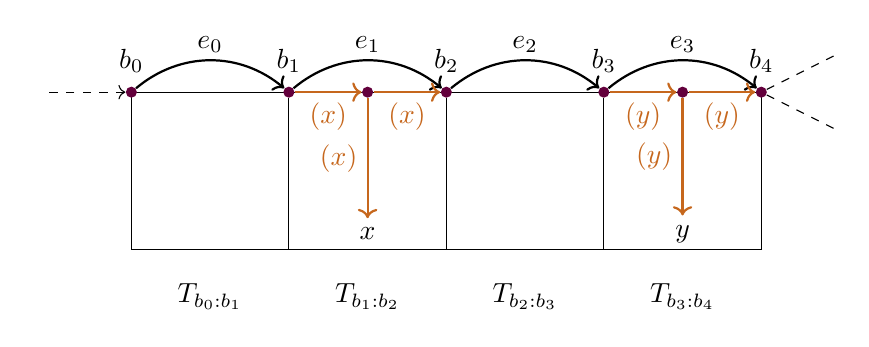
\begin{tikzpicture}[
        localType/.style={
            color=C3,
            thick
        },
        branchProj/.style = {
            color=Prune,
            inner sep=0pt,
            minimum size=4pt,
            fill,
            circle
        },
        leaf/.style={
            color=Prune,
        },
        ]
        \draw (0,0) rectangle (8,2);
        \node (root) at (-1.2,2) {$\treeRoot$};
        \foreach \x in {0,1,2,3,4} {
            \coordinate (n\x) at ({ 2 * \x},0);
            \coordinate (pb\x) at ({ 2 * \x},2);
            \node[branchProj] (b\x) at (pb\x) {};
            \node (lb\x) at ({ 2 * \x},2.4) {$b_{\x}$};
            \draw (n\x) -- (b\x);
        }
        \draw[dashed,<-] (b0) -- (root);
        \draw[dashed] (b4) -- (9,2.5);
        \draw[dashed] (b4) -- (9,1.5);

        \foreach[count=\x] \y in {0,1,2,3} {
            \node (E\x) at ({ 2 * \x - 1},2.6) {$e_{\y}$};
            \draw[->,thick] (b\y) to[bend left=40] (b\x);
            \node (T\x) at ({ 2 * \x - 1},-0.6) {$T_{b_{\y}:b_{\x}}$};
        }
        
        \node (x) at (3,0.2)  {$x$};
        \node (y) at (7,0.2)  {$y$};
        \node[branchProj] (tx) at (3,2) {};
        \node[branchProj] (ty) at (7,2) {};

        \draw[localType, <-] (x)  -- 
        node[midway, left] {$\BtL(x)$} (tx);
        (tx);
        \draw[localType, ->] (tx) -- 
        node[midway, below] {$\BrL(x)$}
        (b2);
        \draw[localType, <-] (tx) -- 
        node[midway, below] {$\BlL(x)$}
        (b1);

        \draw[localType, <-] (y)  -- 
        node[midway, left] {$\BtL(y)$} 
        (ty);
        \draw[localType, ->] (ty) -- 
        node[midway, below] {$\BrL(y)$}
        (b4);
        \draw[localType, <-] (ty) --
        node[midway, below] {$\BlL(y)$}
        (b3);
    \end{tikzpicture}
    }
    \caption{Partitionning a branch of a tree using a \kl{bough}. To compute
    the presence of an edge between $x$ and $y$ in the resulting graph, 
    it is sufficient to know the values of
    $\tlbl{\t}{b_2}{b_3}$, and the respective \kl{bough types} of $x$ and $y$.}
    \label{partitionning-a-graph:fig}
\end{figure}

\AP In the rest of the paper, we will ofter rely on some tree surgery operation
consisting in replacing a \kl{bough} in a tree $\t$ by some other \kl{bough}.
Two boughs $B$ and $B'$ are \intro{compatible} if they start with the same
idempotent value, and if for every tree $\aTree$ that contains $B$, one can
replace $B$ by $B'$ to obtain a new tree $\aTree'$ that remains \kl{forward
Ramseyan}, and conversely for every tree $\aTree'$ that contains $B'$. The
following \cref{fact:bough-replacement} states that one can safely perform such
a replacement without modifying the part of the graph represented by the tree
$\t$ outside of the \kl{bough}.

\begin{fact}
  \label{fact:bough-replacement}
  Let $\t$ be a tree with a \kl{bough} $B$ of level $k$, 
  and let $H$ be a \kl{bough} that is \kl{compatible}
  with $B$. Let $\t'$ be the tree obtained by replacing $B$ by $H$ in $\t$.
  Then, the subraph of $\someInterp(\t)$ induced by the leaves 
  outside of $B$ is isomorphic (using the identity map) 
  to the subgraph of $\someInterp(\t')$
  induced by the leaves outside of $H$.
\end{fact}

\AP Now that we have an understanding of what happens when replacing a
\kl{bough} in a fixed tree, let us study what happens when we do the opposite
operation, i.e., when we chance the ``context'' in which a \kl{bough} is
placed. 

% TODO:
% - a context is a tree with a bough removed, given by a triple (Troot, Tleft, Tright) where
%   where Troot is the tree above the bough with a distinguished leaf where to plug the bough,
%   and Tleft and Tright are the trees below the bough.
% 
% - the context type of a leaf in a context C is given by the values of 
%   paths from the leaf to the root of Tleft resp Tright


Let us define a \intro{context} $C[\square]$ to be a pair of a tree $A$
with a distinguished hole $\square$ that can be filled by another tree, and a
tree $B$ that can be plugged into this hole. Given a tree $T$ with a hole, one
can place it inside a context $C[\square]$ to obtain a new tree $C[T]$ that is
defined by plugging $T$ into the hole of $A$, and plugging $B$ into the hole of
$T$.


\begin{definition}
    \label{good-bough:def}
    Let $B$ be a \kl{bough} of level $k$ in a tree $\t$.
    We say that $B$ is a \intro{good bough} if, 
    there exists a \kl{compatible} \kl{bough} $H$ of level $k$,
    and a map $h \colon \someInterp(\t{[B]}) \to \someInterp(\t{[H]})$
    such that:
    \begin{enumerate}
        \item $h$ is an embedding of graphs,
        \item $h$ is the identity map on leaves outside of $B$,
        \item there exists a block in $H$ that is left untouched 
          by $h$.
    \end{enumerate}
\end{definition}

\AP Therefore, the main combinatorial obstacle to understanding whether or not
a class is \kl{labelled-well-quasi-ordered} is to understand the behaviour of
pairs of nodes $x$ and $y$ that are \kl{dependent}. This is the motivation
for the following construction that studies the behaviour of
consecutive \kl{$k$-neighbourhoods} in a tree.
\subsection{Gap Embedding(s)}

In order to compare two trees equipped with \kl{forward Ramseyan splits}, we
will design an ordering that respects the tree structure as well as the splits.
This is usually called the \intro{gap embedding} relation, originally defined
by Dershowitz and Tzameret \cite{DERSHOWITZ200380}. It was noticed by Freund
\cite{FREU20} that this ordering can be understood as a nested version of
Kruskal's Tree Theorem, and this will be our point of view in the following,
since we will need to slightly adapt the definition to our setting.

\AP Let us consider some $k \in \set{1, \dots, N}$. We will write
$\Trees{\Sigma,k}{X}(Y)$ for the class of trees with labels in $X \times \set{k,
\ldots, N}$ on the internal nodes, labels in $\Sigma$ on the edges, with a
distinguished root, and such that leaves are labelled in $Y$.
It is immediate that $\Trees{\Sigma,k-1}{X}(Y)$ 
is the least fixed point of the following operator:
\begin{equation*}
  F \colon Z \mapsto Y + \Trees{\Sigma,k}{X}(Z) \quad .
\end{equation*}

It was shown in \cite{LOPEZ23} that any such inductive definition gives 
rise to a \kl{well-quasi-order}, obtained by 





Hence, we are in the opposite situation as with the \kl{composition ordering}:
we have a \kl{well-quasi-order} on trees, but we do not know whether the
interpretation $\someInterp$ is order-preserving from trees (with a choice of
split) to graphs. However, when inserting new nodes, we are often able to state
that the value of $\tlbl{\t}{x}{y}$ is preserved provided that $x$ and $y$ are
sufficiently far apart in the \kl{forward Ramseyan split} of the tree, as
stated in the following lemma.

Problems may arise when $x$ and $y$ are too close in the \kl{forward Ramseyan
split}, for instance because they are \kl{one-separated at level $k$}, or
because one inserts new nodes in the first and last part of the path from $x$
to $y$. A typical example of such a situation is illustrated in the case of a
monoid $M$ with two elements $\set{a, b}$ such that $a^2 = b$ and $b$ is
absorbing. Then, replacing an edge $x \treelt y$ labelled with $a$ by two or more
edges will change the value of $\tlbl{\t}{x}{y}$ from $a$ to $b$.

% TODO start with the positive part !
%
% Lemma: one can extend trees with dummy nodes such that all k-neighbourhoods of
% ``importand nodes'' are of bounded size.
%
% Lemma: one can define a quasi-ordering on trees with important nodes that 
% is wqo, and only touches dummy nodes.
%
% Conclude using Lemma 12
%

% Now: the bad part.
% Assume that there are arbitrarily long bad boughs.
% 
% Lemma 1: we can assume that the context is fixed, because 
% there are essentially finitely many contexts.
%
% Lemma 2: we can then color the graphs obtained by fixing the context in
% one color. By 2-WQO, we would obtain a pair of graphs where one embeds
% into the other, but this gives an embedding of bad boughs, which is a contradiction.
%

\section{Existentially Transducing Finite Paths}
\label{sec:interpreting-paths}

In this section, we will be interested in extracting a very regular structure
from a graph class $\mathcal{C}$ that is not \kl{$\forall$-well-quasi-ordered}.
This structure will take two forms, the first one is a combinatorial notion of
\kl{periodic antichain} that can be traced back to \cite[Section 7]{ALM17}, and
the second one is a logical property of \kl{existentially transducing} the
class of all finite paths.

\begin{definition}[Regular Sequence]
  A \intro{regular sequence (of graphs)} is given by a finite graph $G$,
  a labelling function $\lab \colon V(G) \to \Sigma$ for some finite set
  $\Sigma$, and two finite sets $C, F \subseteq \Sigma^2$. It defines
  an infinite set of graphs $\seqof{G^r}[r \geq 1]$ as follows:
  the vertex set of $G^r$ is $V(G) \times \set{1, \ldots, r}$, and there is an edge
  between $(u,i)$ and $(v,j)$ if and only if one of the following holds:
  \begin{itemize}
      \item $(u,v) \in E(G)$ and $i = j$;
      \item $(\lab(u), \lab(v)) \in C$ and $|i - j| = 1$
      \item $(\lab(u), \lab(v)) \in F$ and $|i - j| > 1$.
  \end{itemize}
\end{definition}

It follows from results of the previous section that one can extract
\kl{periodic antichains} from any hereditary class of graphs that is not
\kl{$\forall$-well-quasi-ordered}, answering positively to \cite[Conjecture
2]{ALM17}.

\begin{lemma}
  \label{lem:regular-antichain}
  If a hereditary class of graphs $\Cls$ is not \kl{$\forall$-well-quasi-ordered},
  then it contains a \kl{periodic sequence} $\seqof{G^r}[r \geq 1]$ that is an
  \kl{antichain} for the \kl{labelled induced subgraph} relation.
\end{lemma}
\begin{proof}
  todo aliaume
\end{proof}

\AP Let us now leverage this combinatorial structure to extract a logical
property of the class $\Cls$. Let us recall that an \intro{existential
interpretation} from (labelled) graphs to graphs is given by an existential
first order formula $\phi_{\text{univ}}(x)$ that selects the vertices of the
interpreted graph, an existential first order formula $\phi_{\text{edge}}(x,y)$
that selects the edges of the interpreted graph, and an existential first order
formula $\phi_{\text{dom}}$ that selects the graphs of $\Cls$ on which the
interpretation is defined. The semantics is that for every graph $G \in \Cls$
satisfying $\phi_{\text{dom}}$, the interpreted graph $\mathcal{I}(G)$ has for
vertex set the vertices of $G$ satisfying $\phi_{\text{univ}}$, and has an edge
between two vertices $u,v$ if and only if $G$ satisfies
$\phi_{\text{edge}}(u,v)$ (which is assumed to be symmetric and irreflexive on
the selected vertices). A class $\Cls$ \intro{existentially interprets} a class
$\mathcal{D}$ if there exists an existential interpretation $\someInterp$ from
$\Cls$ to graphs such that $\mathcal{D} \subseteq \someInterp(\Cls)$. We say
that $\Cls$ \intro{existentially transduces} $\mathcal{D}$ if there exists a
finite labelling set $\Sigma$ such that $\Label{\Sigma}{\Cls}$ \kl{existentially
interprets} $\mathcal{D}$.


\begin{lemma}
  \label{lem:paths-transduction}
  Let $\Cls$ be a \kl{periodic antichain} (having the coloring defined) as in 
  \cref{lem:regular-antichain}. Then $\Cls$ \kl{existentially interprets}
  the class of all finite paths.
\end{lemma}
\begin{proof}
  \todo[inline]{\textbf{MAEL ICI}}
\end{proof}

\begin{corollary}
  \label{cor:not-wqo-implies-transducing-paths}
  If a hereditary class of graphs $\Cls$ is not \kl{$\forall$-well-quasi-ordered},
  then it \kl{existentially transduces} the class of all finite paths.
\end{corollary}
\begin{proof}
  \todo[inline]{\textbf{MAEL ICI}}
  It follows from \cref{lem:regular-antichain} and
  \cref{lem:paths-transduction}.
\end{proof}

\begin{conjecture}
  \label{conj:paths-transduction}
  A hereditary class of graphs $\Cls$ is \kl{$\forall$-well-quasi-ordered} if and
  only if it does not \kl{existentially interprets} the class of all finite paths.
\end{conjecture}

This could be 

\section{Structural Graph Theory}

There have been recent results in structural graph theory.

\begin{theorem}[{\cite[Theorem 2.6]{DMT24}}]
    \label{monadically-dependent-patterns:thm}
    Let $\Cls$ be a graph class. Then $\Cls$ is \kl{monadically dependent}
    if and only if for every $r \geq 1$ there exists $k \in \Nat$ such that
    $\Cls$ excludes as \kl{induced subgraphs}:
    \begin{itemize}
        \item all flipped star $r$-crossings of order $k$,
        \item all flipped clique $r$-crossings of order $k$,
        \item all flipped half-graph $r$-crossings of order $k$, and
        \item the comparability grid of order $k$.
    \end{itemize}
\end{theorem}

\begin{corollary}
    \label{wqo-mon-independent:cor}
    Let $\Cls$ be a class of graphs that is 
    \kl{labelled-wqo}. 
    Then $\Cls$ is \kl{monadically dependent}.
\end{corollary}

We go beyond and prove the following class inclusions \kl{labelled-wqo} is
included in \kl{monadically existentially-path free} included in
\kl{monadically dependent}.

\section{Concluding Remarks}
\label{sec:conclusion}

We have proven that for all classes of graphs of bounded clique-width, the
\kl{wqo-wqo} and \kl{labelled-wqo} are two equivalent notions. This result is a
first step towards proving this conjecture for arbitrary classes of graphs.



% Include the bibliography
\bibliographystyle{plainurl}
\bibliography{papers.bib}

% If there are any appendices, we include them here.


\end{document}
